%!TEX root = ../../common/main.tex

\chapter{The \acs*{LHCb} experiment}
\label{ch:lhcb_experiment}

%%%%%%%%%%%%%%%%%%%%%%%%%%%%%%%%%%%%%%%%%%%%%%%%%%%%%%%%%%%%%%%%%%%%%%%%%%%%%%%%
\section{The \acs*{LHC} and its experiments}
\label{ch:lhcb_experiment:lhc}

With a circumference of \SI{26.7}{\kilo\metre} the \LHC is the largest man-made
particle accelerator. Using a \enquote{two-in-one} super-conducting magnet
design, two counter-rotating beams of protons (or ions) are intersected and
brought to collision at four interaction points, home of the large \LHC
experiments \acs*{ALICE}, \acs*{ATLAS}, \acs*{CMS}, and \acs*{LHCb}. The
colliders centre-of-mass energy of $\sqrt{s}=\SI{14}{\TeV}$ and a peak
luminosity of $L=\SI{10e34}{\lumi}$ provide \LHC's experiments with high event
rates that are necessary in their searches for physics beyond the \SM.

Following approval in 1994, the \LHC re-used the existing \LEP tunnel and most
of its infrastructure after \LEP shut down in 2000. The \LHC---and former
\LEP---tunnel is built up of eight straight and eight arc sections and has a
internal diameter of $\SI{3.7}{\metre}$. It is located north-west of Geneva,
Switzerland at a depth between $\SI{45}{\metre}$ and $\SI{170}{\metre}$ below
the surface. The storage ring consists of superconducting NbTi magnets kept at
an operating temperature of $\SI{1.9}{\kelvin}$ by superfluid helium. A
superconducting \RF cavity system captures, accelerates, and stores the two
proton beams.

At design luminosity $\num{2808}$ bunches with a bunch spacing of
$\SI{25}{\nano\metre}$ are stored in each proton beam. The \LHC relies on a
supply chain of smaller accelerators providing the initial proton bunches.
\Cref{fig:lhcb_experiment:lhc:cern_accelerator_complex} depicts the \acs{CERN}
accelerator complex. A bottle of hydrogen gas is the source of the protons, that
are then subsequently accelerated to higher energies by the \LINACTwo, the
\BOOSTER, the \PSyn, and the \SPS, before being injected into the \LHC at an
energy of $\SI{450}{\GeV}$. The transfer lines Tl2 and Tl8 are used to inject
the protons bunches in both beam directions. As soon as the nominal number of
proton bunches is reached, the beam energies are increased up to $\SI{7}{\TeV}$
for each beam. The average \LHC turnaround time, \ie the time it takes to run
through the whole accelerator chain until a stable beam is achieved, adds up to
seven hours. Mainly due to beam loss from \pp collisions the beam intensities
and the instantaneous luminosity decays. Starting from a peak luminosity of
$L=\SI{10e34}{\lumi}$ a luminosity lifetime of 15 hours is estimated. To prevent
uncontrolled beam losses and to protect the \LHC infrastructure and the \LHC
experiments a beam dump system is installed. The fully automated system monitors
the beam condition and is able to extract the beam from the \LHC using kicker
magnets in case of a failure. The beam dump system is also used regularly to
extract the beam after a successful run.

\begin{figure}[t]
  %% trim={<left> <lower> <right> <upper>}
  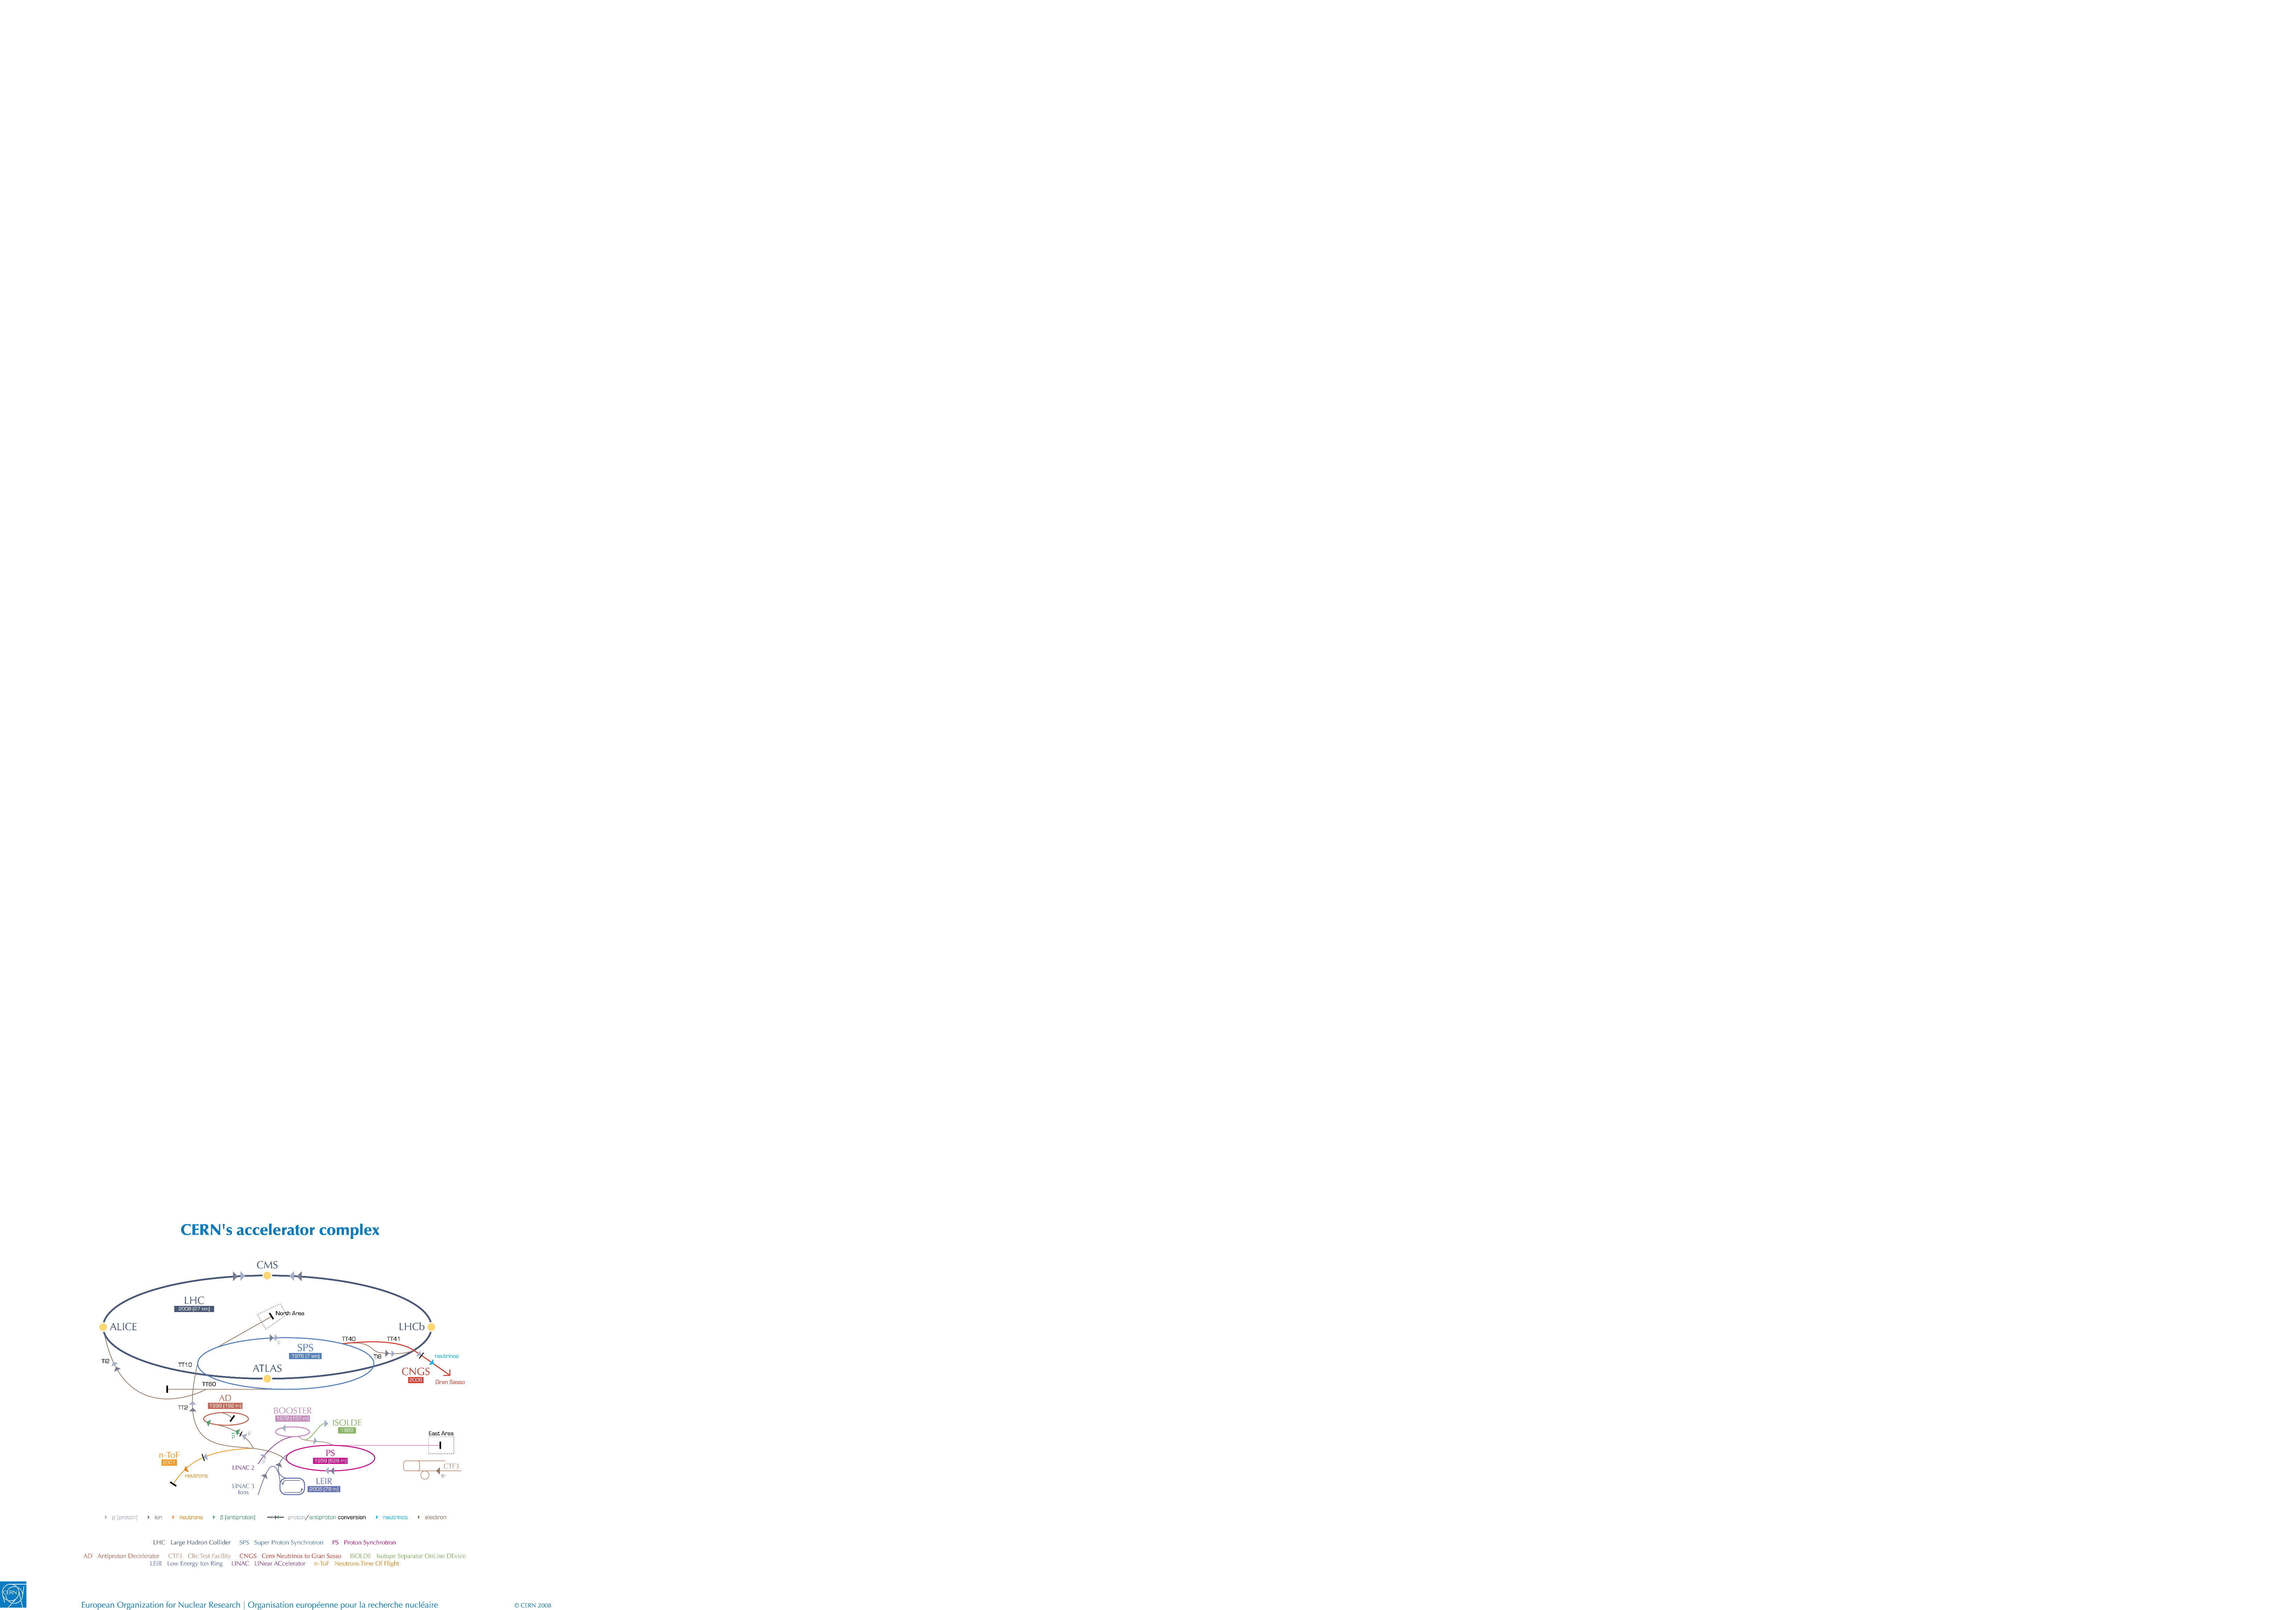
\includegraphics[width=\textwidth, trim={4.8cm 5.3cm 4.2cm 1.8cm}, clip=true]{private/content/the-lhcb-experiment/figs/cern_acceleator_complex.pdf}
  \caption{
  The \acs{CERN} accelerator complex \cite{Christiane:1260465}.\todo{Highlight that Fig. is modified} 
  Starting from the \acs{LINACTwo}, protons are accelerated through the
  \acs{BOOSTER}, the \acs{PSyn} and finally the \acs{SPS} before being injected
  into the \LHC. If one or both beams consist of heavy ions, the
  \acs*{LINACThree} and the \acs*{LEIR} are used to accelerate the ions and inject
  them into the \acs{PSyn}.
  }
  \label{fig:lhcb_experiment:lhc:cern_accelerator_complex}
\end{figure}

Shortly after the first successful circulation of two proton beams in September
2008, a fault occurred in the electrical bus connection between two magnets,
leading to a large helium leak and serious damage to several of \LHC's magnets
and infrastructure. After the incident, the management decided to reduce the
beam energy and intensity. Thus, in the years 2010 and 2011 the \LHC
centre-of-mass energy was $\sqrt{s}=\SI{7}{\TeV}$ with a bunch spacing of
$\SI{50}{\nano\metre}$ delivering a peak instantaneous luminosity of
$\SI{2.4e33}{\lumi}$. An increase of the beam energy to $\sqrt{s}=\SI{8}{\TeV}$
lead to a peak instantaneous luminosity of $\SI{7.7e33}{\lumi}$ in 2012
\cite{Lamont:2013cma}.

The \LHC is not only capable of colliding protons but also lead ions in Pb-Pb
as well as in \proton-Pb and Pb-\proton collisions. For this purpose the \ALICE
detector \cite{Aamodt:2008zz} is specifically designed to study QCD interactions
and the quark-gluon plasma produced in the \LHC ion runs, where it has to cope
with very large particle multiplicities. In the case of an heavy ion run, the
\LINACThree and the \LEIR mark the starting point of the accelerator chain,
before injecting the lead ions into the \PSyn.

In total, seven experiments are located at the four interaction regions of the
\LHC. The two multi-purpose detectors \ATLAS \cite{Aad:2008zzm} and \CMS
\cite{Chatrchyan:2008aa} are installed at opposite sides of the storage ring.
Both experiments cover a great variety of physics activities: the search for
scalar particles, particles predicted by super-symmetric models, dark matter
candidates, and evidence for extra spacial dimensions. Around the interaction
regions of the \CMS experiment, the \TOTEM detectors \cite{Anelli:2008zza} are
located. Together with the \LHCf experiment \cite{Adriani:2008zz}, located on
both sides of the \ATLAS interaction region, the detectors are designated to
address the study of the \enquote{forward} region of the collisions at very
small angles to the beam direction. The seventh experiment \MoEDAL extends the
\LHC physics program to the direct search for magnetic monopoles. Still missing
in this list, is the \LHCb experiment, that will be explained in more detail in
the next section.

% to enforce definition of abbreviations
\acuse{LINACThree,LEIR,ALICE,ATLAS,CMS,TOTEM,MoEDAL,LHCf}

%%%%%%%%%%%%%%%%%%%%%%%%%%%%%%%%%%%%%%%%%%%%%%%%%%%%%%%%%%%%%%%%%%%%%%%%%%%%%%%%
\section{The LHCb detector}
\label{ch:lhcb_experiment:detector}

The \LHCb detector is a unique precision instrument solely designed to study \CP
violation and rare decays of beauty and charm hadrons. He is constructed as a
single-arm spectrometer covering an angular range from approximately
$\SI{10}{\mrad}$ to $\SI{300}{\mrad}$ ($\SI{250}{\mrad}$) in the
horizontal (vertical) plane.

The detector layout exploits the characteristics of the heavy flavour production
in \protonproton collisions at the \LHC. The production of heavy quarks in an
hadronic environment is dominated by gluon-gluon fusion and quark-antiquark
annihilation.

\info{Better understand how b quark production works at the LHC}
bbbar production process:
hadrons, PDF, gluon-gluon fusion

b hadron production: large number of b/c hadrons, bbbar crosssection, asymmetric
momentum distribution (plots!), hadronization into Bd, Bs, Bu, baryons;
production asymmetry

lumi leveling, angular acceptance, number of B decays in acceptance

%%%%%%%%%%%%%%%%%%%%%%%%%%%%%%%%%%%%%%%%%%%%%%%%%%%%%%%%%%%%%%%%%%%%%%%%%%%%%%%%
\section{Track reconstruction}
\label{ch:lhcb_experiment:tracking}

The \LHCb track reconstruction is based on information from a set of tracking
detectors: the \VELO, the \TT, the \IT and the \OT. Silicon microstrips are used
in the first three, while the latter is constructed as a straw-tube detector.
The \VELO is described in \cref{ch:lhcb_experiment:tracking:velo}, the \TT and
the \IT in \cref{ch:lhcb_experiment:tracking:ttit}, and the \OT in
\cref{ch:lhcb_experiment:tracking:ot}.

%%------------------------------------------------------------------------------
\subsection{The \acl*{VELO}}
\label{ch:lhcb_experiment:tracking:velo}

Surrounding the \protonproton interaction region the \VELO's main purpose is the
precise position measurement of traversing particles to reconstruct the \ac{PV}
and displaced \acp{SV}. To achieve the best possible spatial resolution the
sensors must be positioned close to the beam trajectory. To allow the sensors to
be as close as $\SI{8}{\milli\metre}$ to the interaction region and still
prevent damage during beam injection, the \VELO modules are split in two halves
an can be retracted until stable beams are present. Each single modules consists
of two half-disk shaped silicon microstrip sensor modules covering either the
radial dimensions ($R$ sensor) or the angular dimension ($\Phi$ sensor) as can
be seen in the schematic visualisation in
\cref{fig:lhcb_experiment:tracking:velo:sensor}.
%
\begin{figure}[t]
  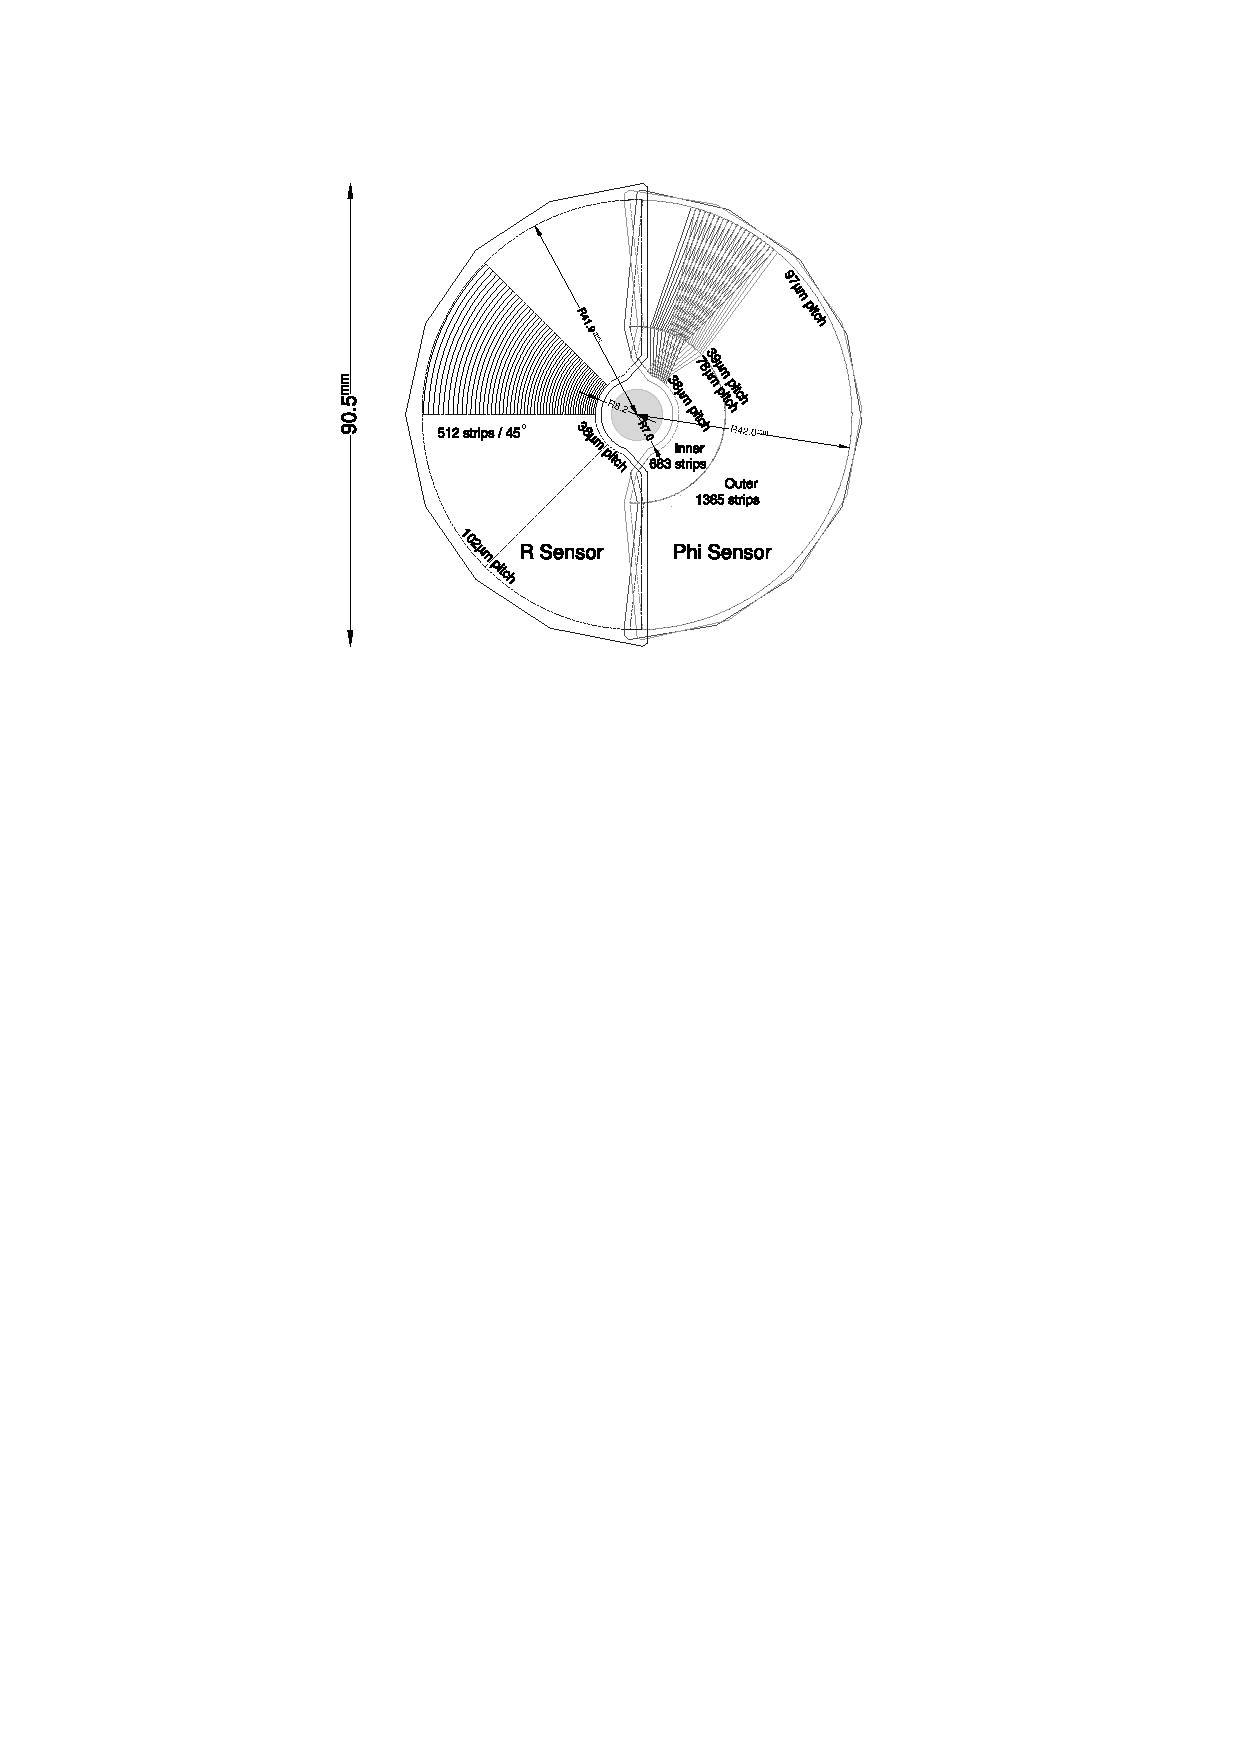
\includegraphics[width=0.42\textwidth]{private/content/the-lhcb-experiment/figs/lhcb_detector_velo_sensors.pdf}
  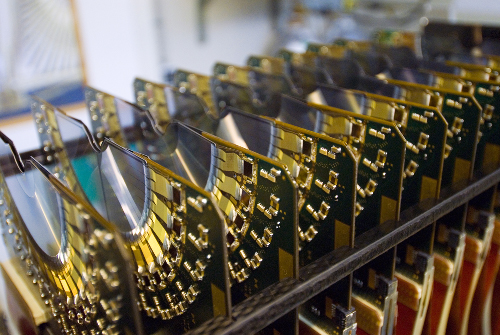
\includegraphics[width=0.55\textwidth]{private/content/the-lhcb-experiment/figs/lhcb_detector_velo_assembly.jpg}
  \caption{(Left) Schematic representation of the $R$ and $\Phi$ sensor for one
  of the \VELO modules \cite{Alves:2008zz}. (Right) Picture of the \VELO during
  assembly \cite{Aaij:1707015}. }
  \label{fig:lhcb_experiment:tracking:velo:sensor}
\end{figure}
%
The \VELO covers the total \LHCb acceptance region, such that all tracks cross
at least three \VELO stations. \Cref{fig:lhcb_experiment:tracking:velo:overview}
shows the cross section of the \VELO in the $(x,z)$ plane at $y=0$ with all
modules visible. \info{VELO pile-up system?}
%
\begin{figure}[t]
  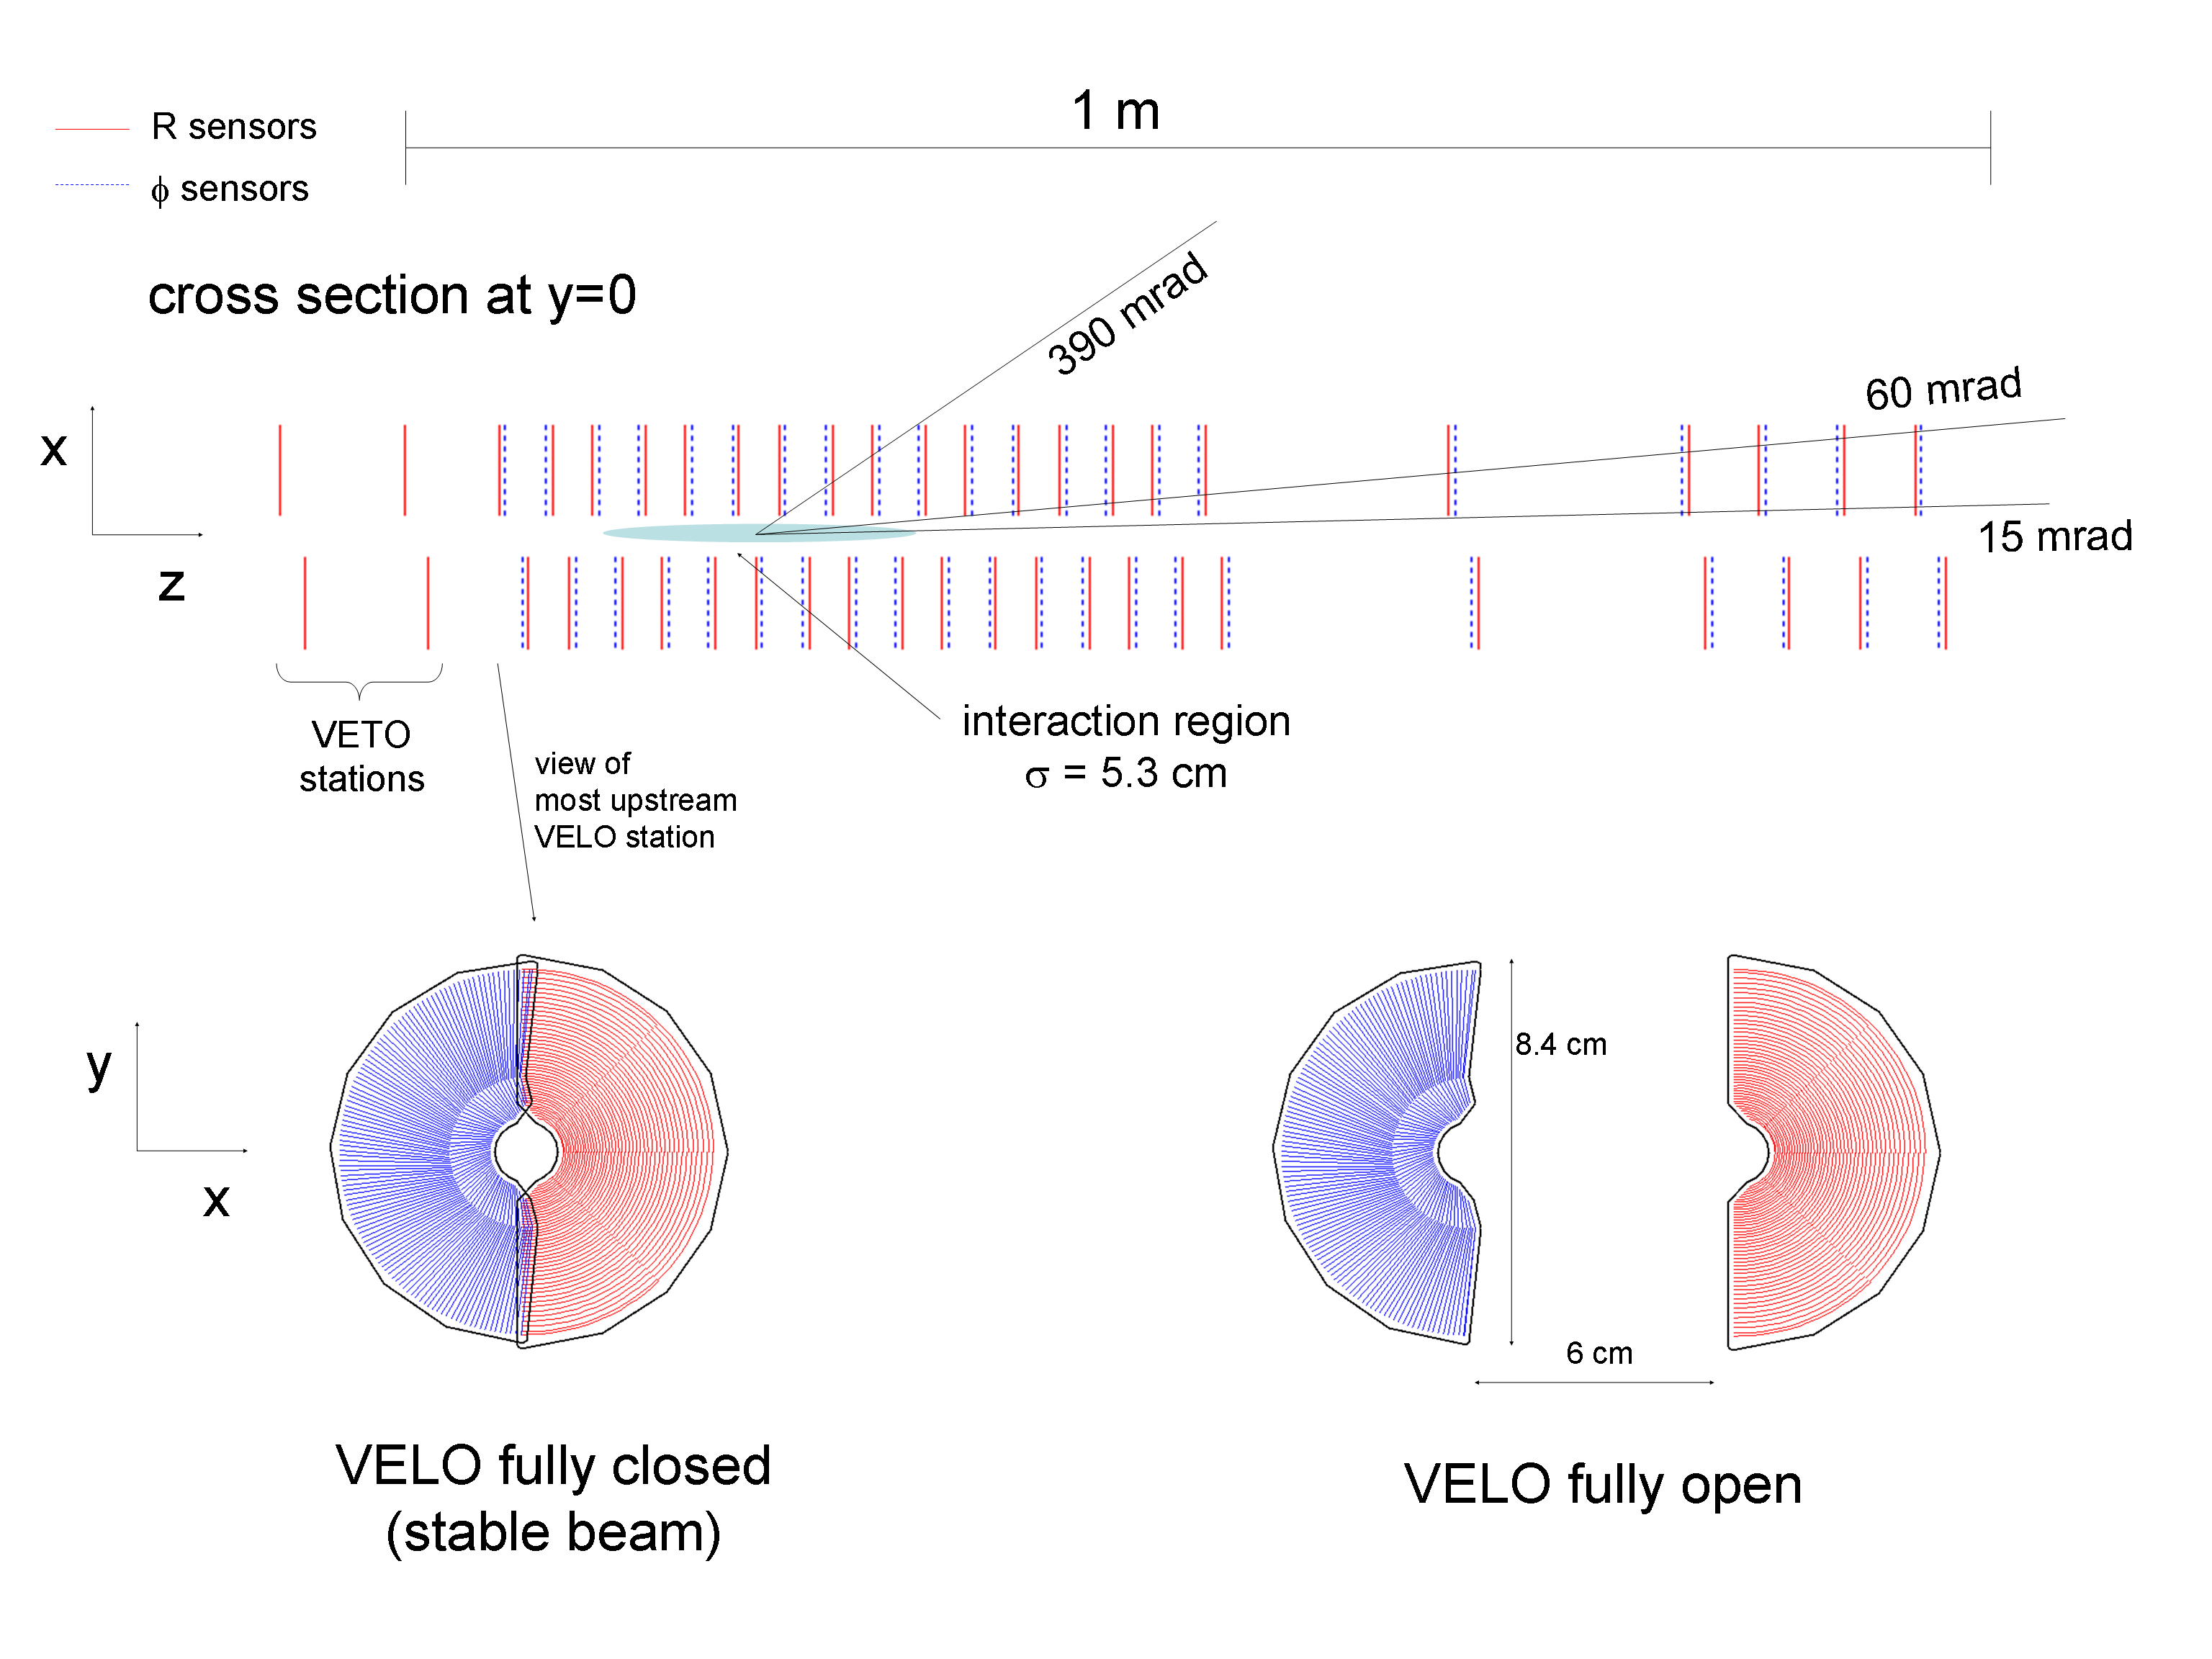
\includegraphics[width=\textwidth]{private/content/the-lhcb-experiment/figs/lhcb_detector_velo_overview.png}
  \caption{
    Cross section of the closed \VELO in the $(x,z)$ plane at $y=0$ \cite{Alves:2008zz}.
  }
  \label{fig:lhcb_experiment:tracking:velo:overview}
\end{figure}

% \begin{itemize}
%   \item purpose: displaced secondary vertices, decay length, decay time, IP
%   \item silicon modules in r and phi, geometrical dimensions, mechanical accuracy, closest approach to beam
%   \item acceptance: 1.6 < eta < 4.9; |z| < 10.6cm
%   \item requirement of at least three hits in the VELO stations
%   \item pile-up veto system
%   \item retractable, RF foil, in vacuum (primary and secondary)
%   \item hardware interlock system
%   \item performance(?)
% \end{itemize}
%%------------------------------------------------------------------------------
\subsection{TT \& IT}
\label{ch:lhcb_experiment:tracking:ttit}
\begin{itemize}
  \item silicon microstrip sensors
  \item position, geometrical dimensions, active area, x-u-v-x alignment
  \item TT pros: spatial resolution, hit occupancy, signal shaping time, single-hit efficiency, radiation damage, material budget, number of readout channels
  \item IT parts: ...
\end{itemize}
%%------------------------------------------------------------------------------
\subsection{OT}
\label{ch:lhcb_experiment:tracking:ot}
\begin{itemize}
  \item drift-time detector, tracking of charged particles
  \item array of gas-tight straw-tube modules, each module two layers of drift-tubes
  \item drift-time < 50ns, drift-coordinate resolution 200mum
  \item three stations, each of four layers in x-u-v-x alignment, gas admixture, acceptance
\end{itemize}
%%------------------------------------------------------------------------------
\subsection{Muon}
\label{ch:lhcb_experiment:tracking:muon}
\todo{Decide if the muon system belongs to tracking or PID}
\begin{itemize}
  \item five stations of multi-wire proportional chambers
  \item muon ID important for charmonium final states and rare decays
  \item high pT trigger for L0, and muon ID for HLT
\end{itemize}
%%------------------------------------------------------------------------------
\subsection{Track reconstruction technique and performance}
Results are form Bd2JpsiKS!
\begin{itemize}
  \item hits from VELO, TT, IT and OT are combined to form trajectories form the VELO to the calorimeters. 
  \item list different track types: long, upstream, downstream, VELO, T
  \item track seeds, Kalman filter, pattern recognition, ghosts
  \item definition of: reconstructible, successfully reconstructed
  \item performance numbers for long tracks and downstream tracks
\end{itemize}

%%%%%%%%%%%%%%%%%%%%%%%%%%%%%%%%%%%%%%%%%%%%%%%%%%%%%%%%%%%%%%%%%%%%%%%%%%%%%%%%
\section{Particle identification}
\label{ch:lhcb_experiment:pid}
%%------------------------------------------------------------------------------
\subsection{RICH}
\begin{itemize}
  \item general: cherenkov light detectors, spherical and flat mirrors, hybrid photon detectors
  \item RICH1: low momentum charged particles, 1-60GeV/c, aerogel and C4F10 radiators
  \item RICH2: CF4 gas radiator, 15-100GeV/c, reduced polar angle acceptance
  \item HPDs: 
\end{itemize}
%%------------------------------------------------------------------------------
\subsection{Calo}
\begin{itemize}
  \item trigger tasks: transverse energy hadron/electron/photon candidates for L0
  \item PID for electrons, photons, hadrons
  \item energy and position measurement
  \item design: ECAL (+SPD and PS), HCAL
  \item technical details: create scintillation light, then transmit to a photo-multiplier using fibres
\end{itemize}
%%------------------------------------------------------------------------------
\subsection{Particle identification technique and performance}
\begin{itemize}
  \item combine info from RICHs, calo, and muon system to identify: e,mu,pi,K,p also gamma, pi0
  \item hadron PID: likelihood approach, RICH pattern mached to all possible tracks under assumption of partice hypotheses. -> global pattern-recongnition
  \item RICH efficiency
  \item muon PID: extrapolating reconstructed tracks into the muon stations; considered a muon cand if a minimum number of stations have hits in their field of interest FOI
  \item muon PID efficiency
  \item lectron PID: balance of track momentum and energy of the charged cluster in the ECAL matched with extrapolated tracks; matching bremsstrahlung photons to electron tracks before the magnet
  \item gamma PID: ECAL cluster w/o associated track
  \item pi0 PID: 
  \item global performance: PV resolution of 10mum transverse to the beam and 60mum along the beam axis; invariant mass resolution between 12 and 25 MeV; lifetime resolution of around 40fs
\end{itemize}

%%%%%%%%%%%%%%%%%%%%%%%%%%%%%%%%%%%%%%%%%%%%%%%%%%%%%%%%%%%%%%%%%%%%%%%%%%%%%%%%
\section{Trigger}
two level trigger system: L0 and HLT, L0 from custom made electronics, real-time with bunch crossing-frequency, HLT on software in processor farm
%%------------------------------------------------------------------------------
\subsection{L0 trigger}
from 40MHz to 1MHz, trigger on large transverse momentum pT and energy ET; the hightest ET hadron, electron, photon clusters in the calo; the two highest pT muons in the muon chambers; pile-up system in velo calculates the number of PVs; the caos calculate the total observed energy and estimate the number of tracks based on the number of hits in the SPD; using these global event cuts to reject events which would otherwise be triggered due to large combinatorics
%%------------------------------------------------------------------------------
\subsection{High level trigger}
reduced the 1MHz L0 output rate to 5kHz; software based and flexible, again composed of two parts: HLT1 and HLT2; 
%%%%%%%%%%%%%%%%%%%%%%%%%%%%%%%%%%%%%%%%%%%%%%%%%%%%%%%%%%%%%%%%%%%%%%%%%%%%%%%%
\section{Online system}
\DAQ, \TFC, and \ECS
\begin{itemize}
  \item \DAQ: transport of bunch-crossing data from the detector fond-end electornics to permanent storage
  \item Front-end detector electronics -> TELL1 board : receiver cards -> \acp{FPGA} (processing, zero-suppresion, data compression) -> SyncLink (another \FPGA) collect and send raw IP-packet by GbEthernet mezzanine cards -> DAQ
  \item TELL1 has a credit-card size PC connected that interfaces to the \ECS
  \item Clock and synchronisation signals (\eg triggers) are transmitted trough the on-board \TTC interface
\end{itemize}

%%%%%%%%%%%%%%%%%%%%%%%%%%%%%%%%%%%%%%%%%%%%%%%%%%%%%%%%%%%%%%%%%%%%%%%%%%%%%%%%
\section{Software stack}
\begin{itemize}
  \item \Gaudi: LHCb software framework (used by ATLAS as well)
  \item \Brunel: reconstruction
  \item \Brunel: trigger
  \item \DaVinci: end-user analysis software
  \item Simulation: \Gauss, \Boole, \Pythia, \EvtGen, \Photos, \Herwigpp, \Sherpa, \GeantFour
\end{itemize}
%%%%%%%%%%%%%%%%%%%%%%%%%%%%%%%%%%%%%%%%%%%%%%%%%%%%%%%%%%%%%%%%%%%%%%%%%%%%%%%%
\section{Computing grid}
...
